\hypertarget{AstuMath_8h}{}\section{include/\+Astu\+Math.h File Reference}
\label{AstuMath_8h}\index{include/\+Astu\+Math.\+h@{include/\+Astu\+Math.\+h}}


This file defines public functions, templates and classes, offered by the mathematics module of A\+S\+T-\/\+Utilities.  


{\ttfamily \#include \char`\"{}Math/\+Vector2.\+h\char`\"{}}\newline
{\ttfamily \#include \char`\"{}Math/\+Vector3.\+h\char`\"{}}\newline
{\ttfamily \#include \char`\"{}Math/\+Matrix3.\+h\char`\"{}}\newline
{\ttfamily \#include \char`\"{}Math/\+Transform2.\+h\char`\"{}}\newline
{\ttfamily \#include \char`\"{}Math/\+Polygon.\+h\char`\"{}}\newline
{\ttfamily \#include \char`\"{}Math/\+Line2.\+h\char`\"{}}\newline
{\ttfamily \#include \char`\"{}Math/\+Ray2.\+h\char`\"{}}\newline
{\ttfamily \#include \char`\"{}Math/\+Segment1.\+h\char`\"{}}\newline
{\ttfamily \#include \char`\"{}Math/\+Segment2.\+h\char`\"{}}\newline
{\ttfamily \#include \char`\"{}Math/\+Random.\+h\char`\"{}}\newline
{\ttfamily \#include \char`\"{}Math/\+Interpolator.\+h\char`\"{}}\newline
Include dependency graph for Astu\+Math.\+h\+:\nopagebreak
\begin{figure}[H]
\begin{center}
\leavevmode
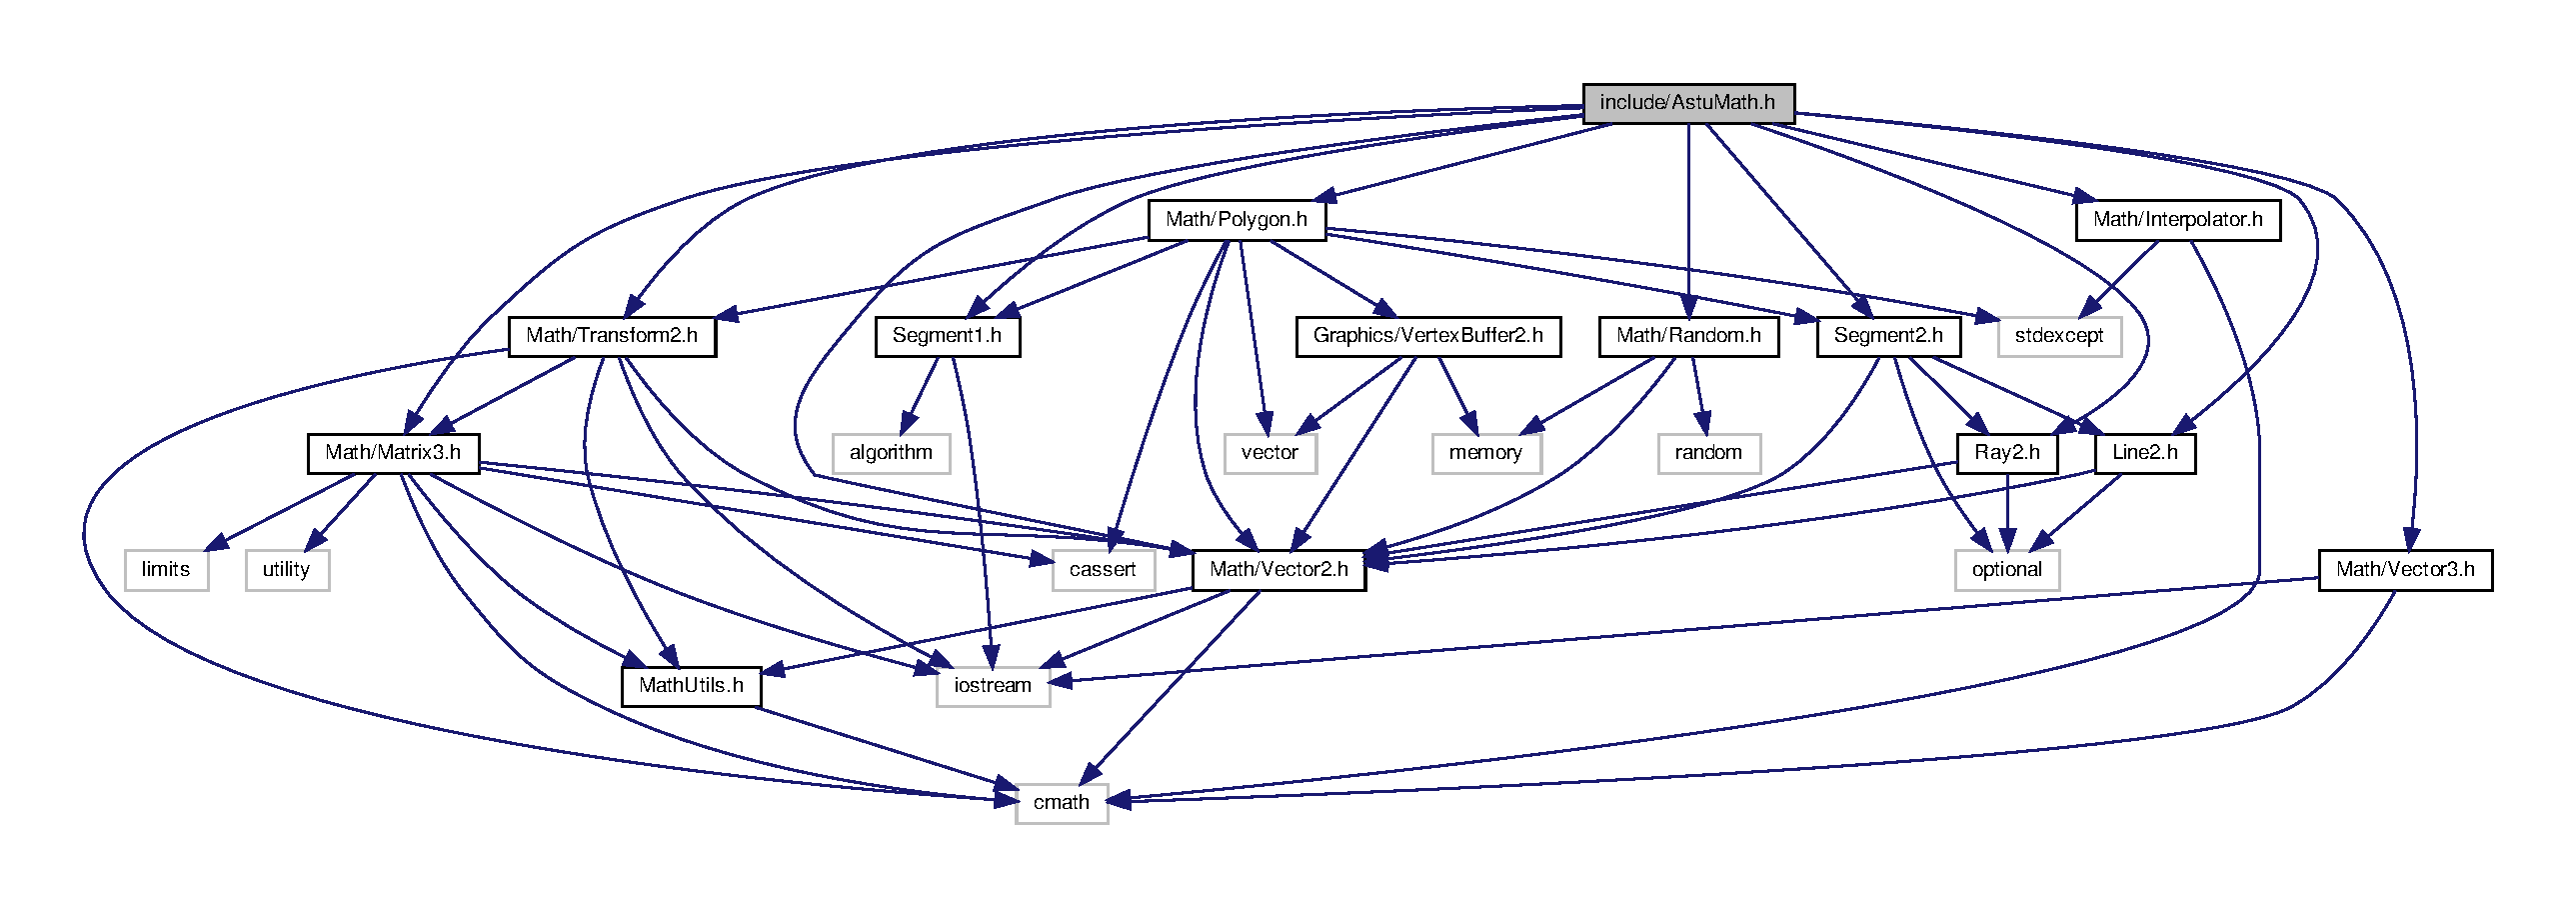
\includegraphics[width=350pt]{AstuMath_8h__incl}
\end{center}
\end{figure}


\subsection{Detailed Description}
This file defines public functions, templates and classes, offered by the mathematics module of A\+S\+T-\/\+Utilities. 

